\section{Results}

\subsection{Ranking of Individual IQA Metrics}

The correlation analysis between individual IQA metrics and MOS revealed significant variability in their predictive performance. Fig.~\ref{fig:ranking} presents a ranked comparison of the 41 evaluated IQA metrics based on the arithmetic mean of the Pearson and Spearman correlation coefficients. Metrics such as MS-SSIM, SAM, and PSNR-B~\cite{ma2011psnr} demonstrated the highest correlation with MOS, suggesting that these metrics consistently align with subjective perception of distortions in facial images.

\begin{figure}[htbp]
    \centering
    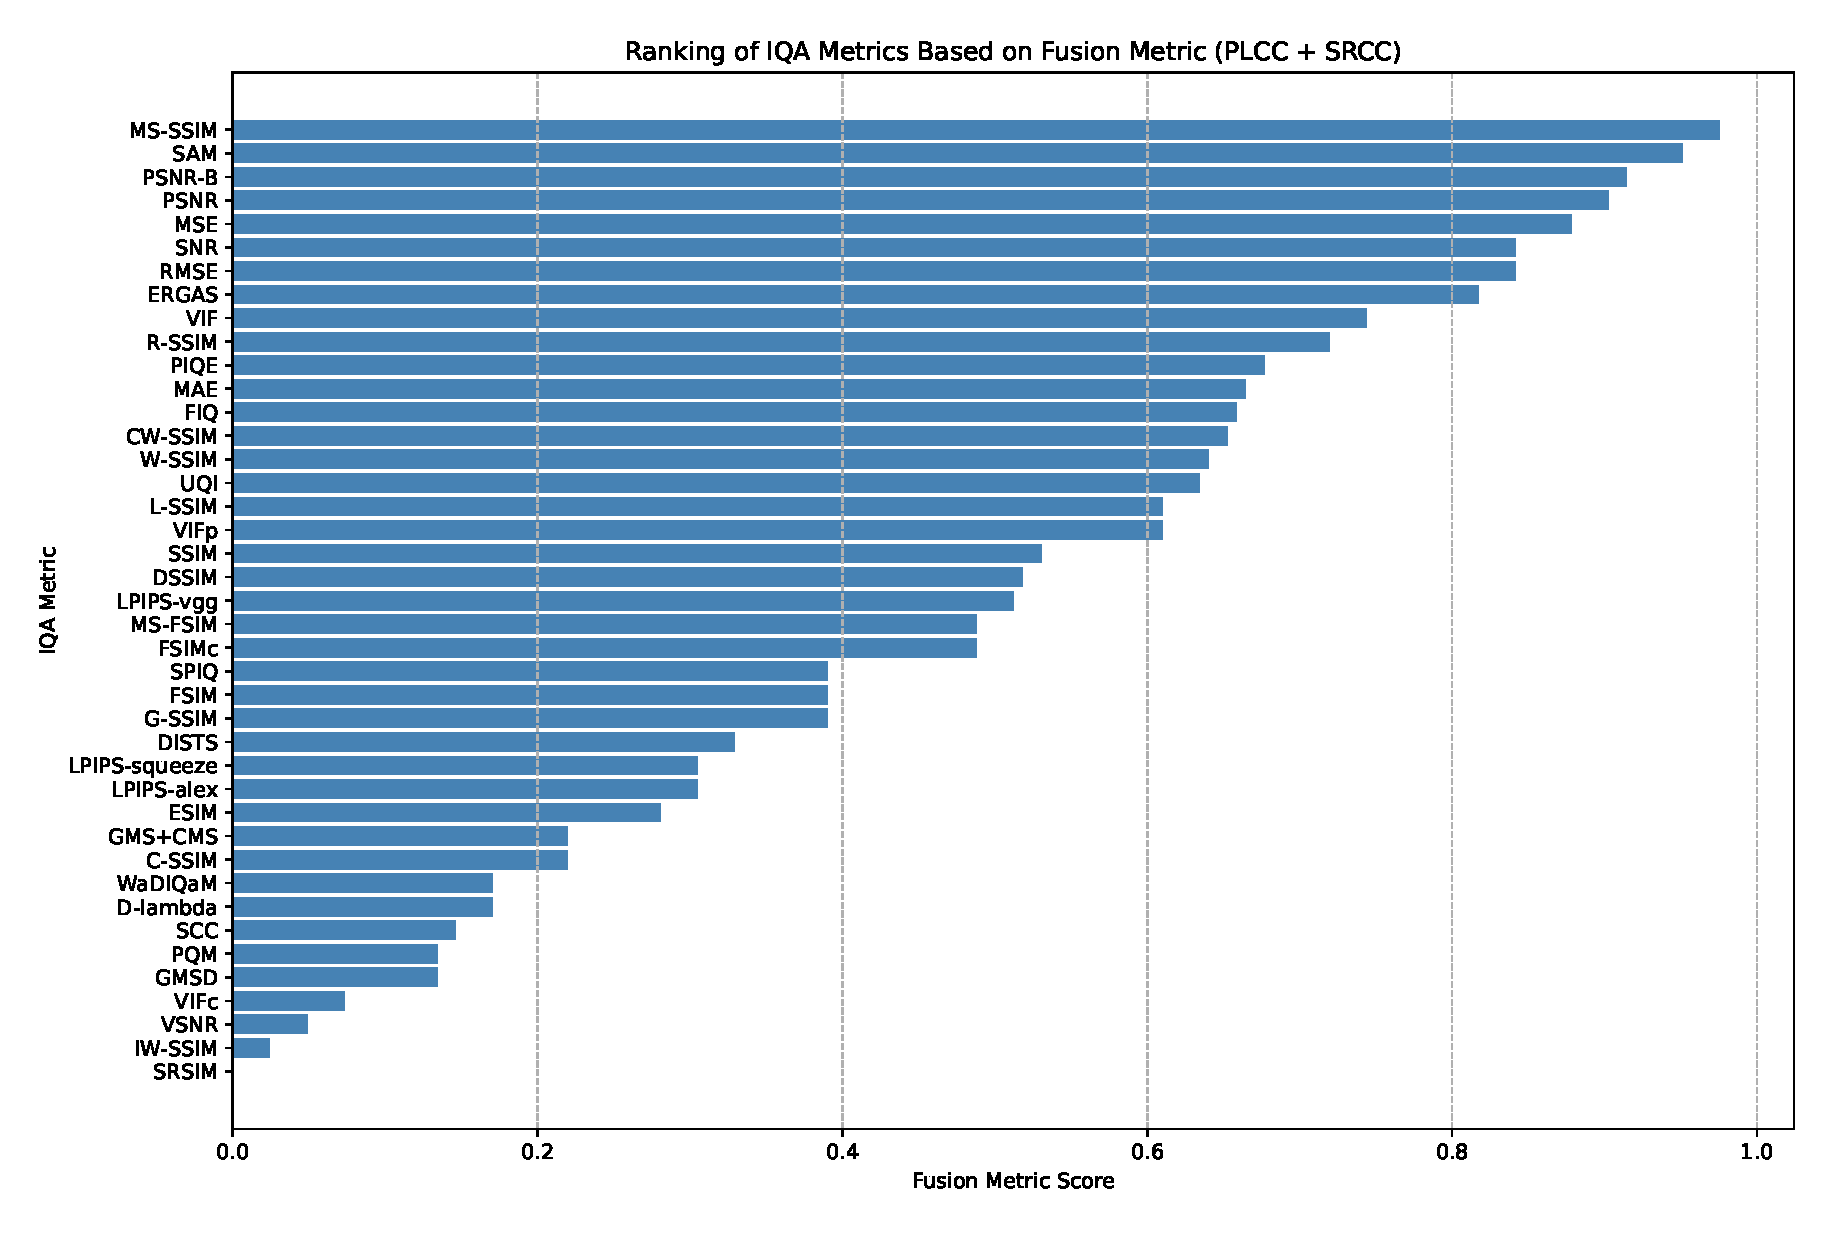
\includegraphics[width=\linewidth]{images/fusion_metric_ranking.eps}
    \caption{Ranking of IQA Metrics Based on Fusion Metric (PLCC \& SRCC).}\label{fig:ranking}
\end{figure}

\subsection{Comparison of Fusion Models}

To evaluate the effectiveness of different fusion techniques, we compared multiple approaches, including PCA-based fusion, ridge regression, and random forest-based models. Fig.~\ref{fig:fusion_vs_mos} summarizes the performance of these models in terms of PLCC and SRCC, indicating that the random forest fusion method yielded the highest correlation with MOS.\@

The results indicate that machine learning-based fusion techniques outperform statistical fusion approaches such as PCA and regression. The random forest fusion model effectively captures nonlinear interactions between IQA metrics, enabling more accurate predictions of subjective image quality. PCA, while useful for dimensionality reduction, discards some potentially valuable information, leading to lower correlation coefficients. Regression-based models, constrained by their linear nature, also fall short in capturing complex dependencies among IQA metrics.

\begin{figure}[htbp]
    \centering
    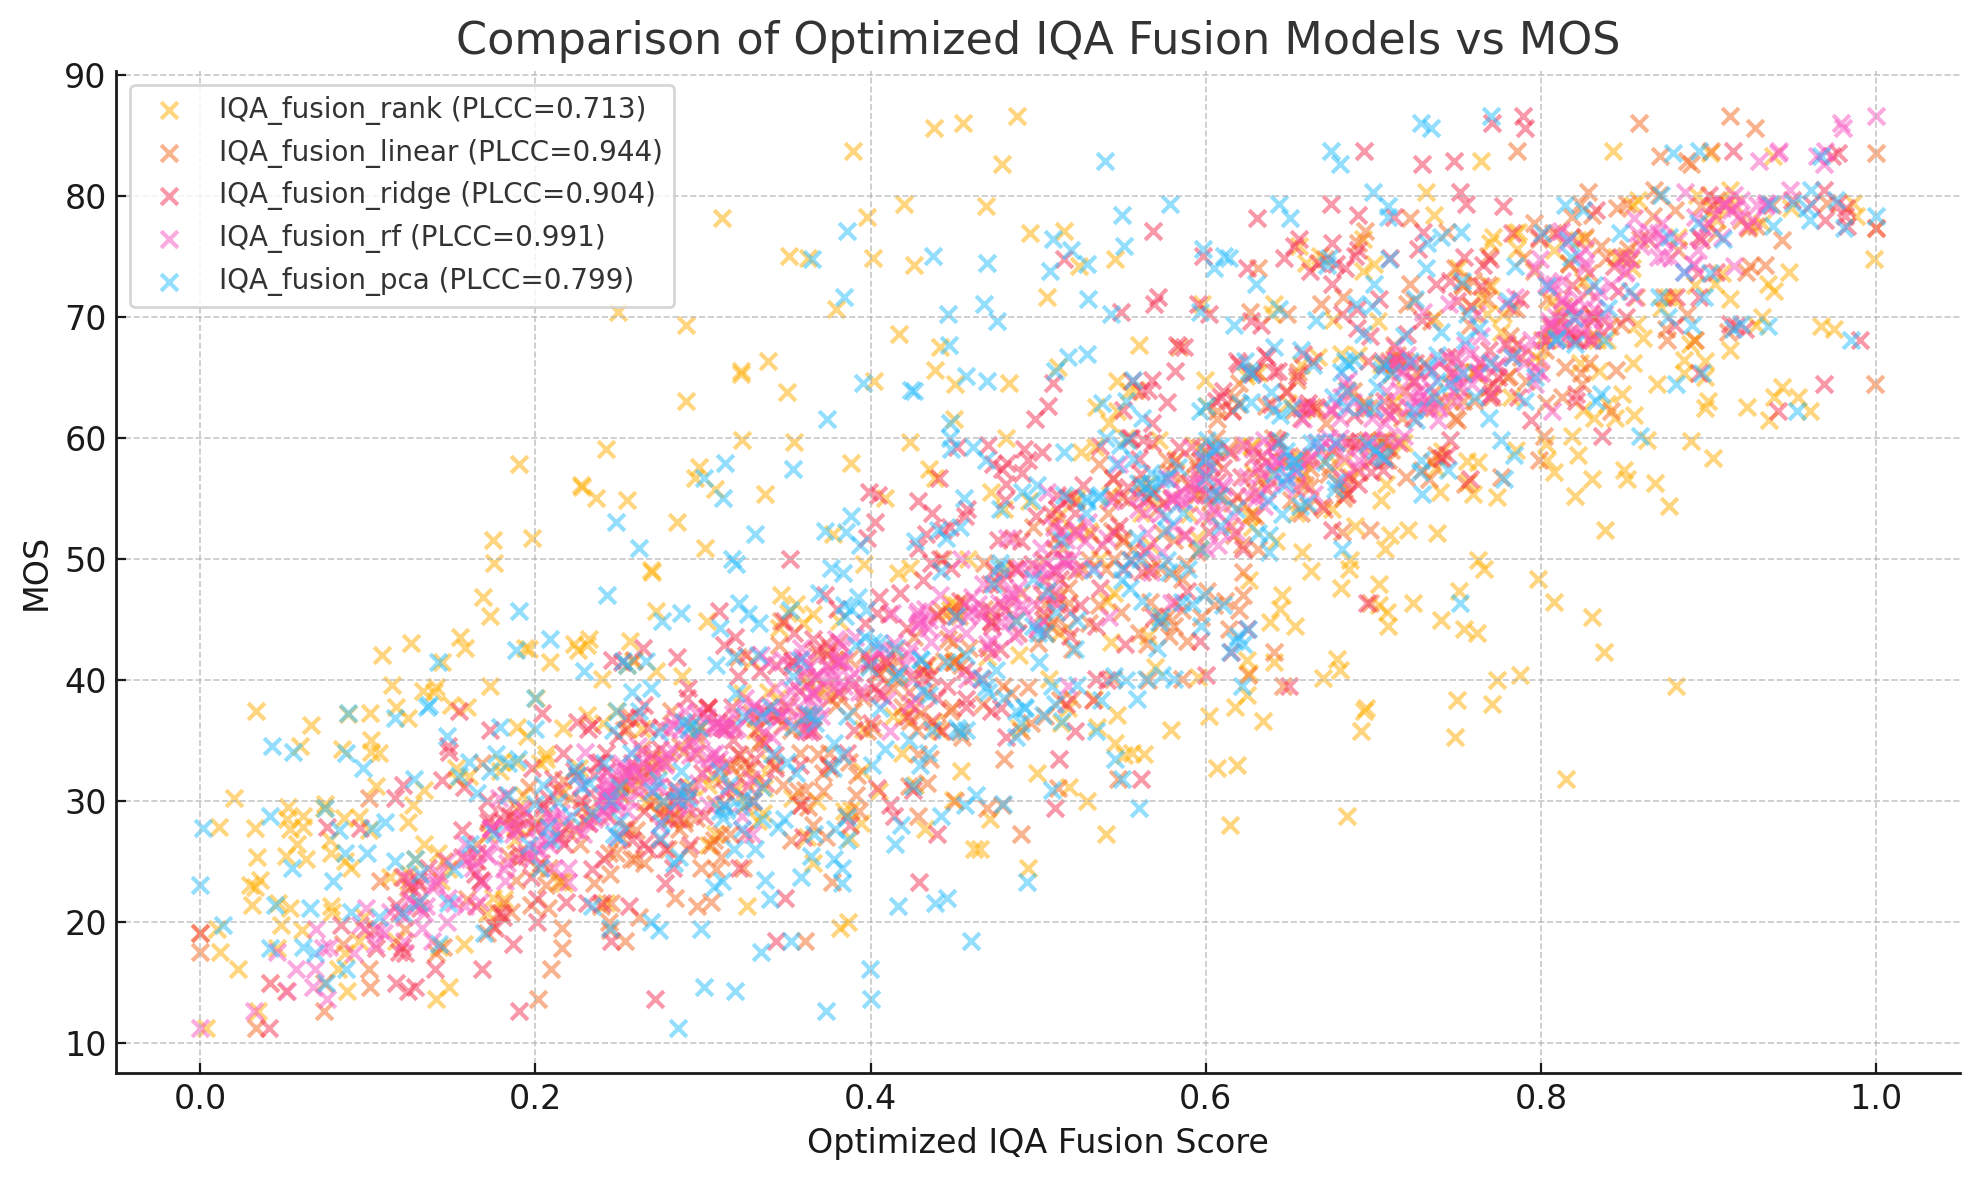
\includegraphics[width=\linewidth]{images/fusion_model_vs_mos.png}
    \caption{Scatter plot of Fusion-Based IQA Scores vs. MOS.}\label{fig:fusion_vs_mos}
\end{figure}

\subsection{Correlation Between Fusion Scores and MOS}

The application of fusion models significantly improved the correlation between IQA scores and MOS.\@ Fig.~\ref{fig:final_comparison_grid} illustrates the relationship between the optimized fusion scores and MOS values, demonstrating a substantial improvement in correlation coefficients.
While deep learning models could further enhance performance, the Open Source Face Image Quality (OFIQ) framework prioritizes simple and fast implementations, making it the most suitable choice for this study.

These results underscore the advantage of integrating multiple IQA metrics to obtain a more reliable predictor of MOS.\@ The success of the fusion model suggests that no single IQA metric is sufficiently comprehensive to capture the full range of perceptual quality factors, but rather, a combination of complementary metrics provides the most robust estimation.

Overall, the findings highlight the superiority of machine learning-based fusion strategies in FIQA.\@ The improved MOS predictability achieved through fusion further supports the hypothesis that integrating multiple complementary metrics enhances the robustness of IQA systems. Additionally, these results provide insights into the design of more accurate quality assessment models that align better with human perception.

\begin{figure}[htbp]
    \centering
    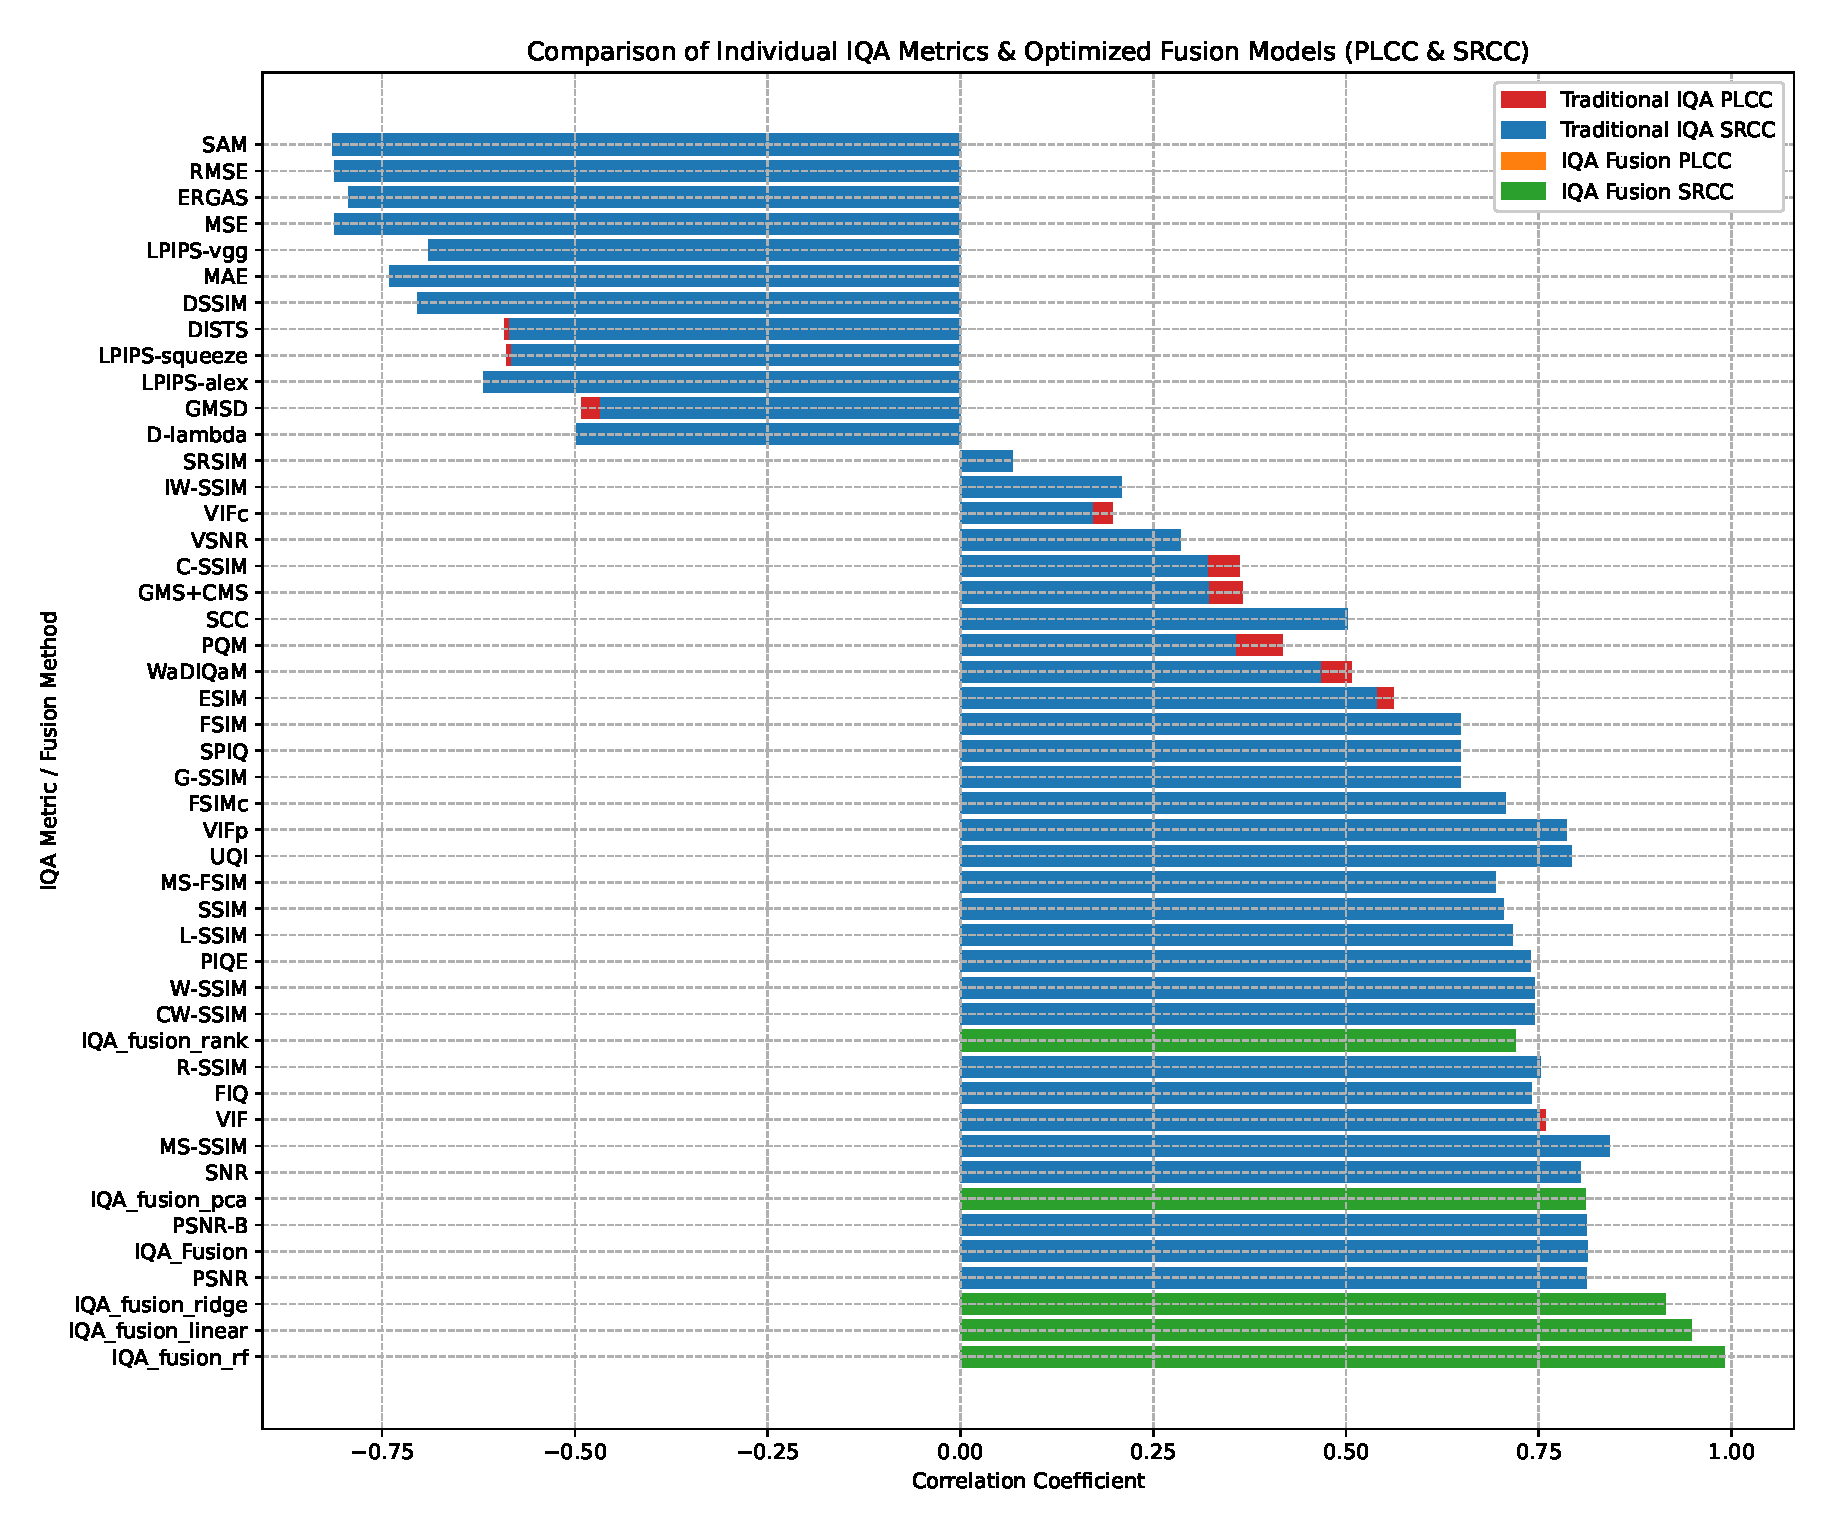
\includegraphics[width=\linewidth]{images/iqa_vs_fusion_iqa.eps}
    \caption{Comparison of IQA metrics and Optimized Fusion Models (PLCC \& SRCC)}\label{fig:final_comparison_grid}
\end{figure}